
\addcontentsline{toc}{section}{Exercițiul 11}
\section*{11. Crearea tabelelor in SQL si inserarea de date coerente in fiecare dintre acestea.}

\vspace{1cm}

\begin{itemize}

    \item \textbf{FIRMA}
    \vspace{0.2cm}
    \begin{lstlisting}
CREATE TABLE FIRMA (
 id_firma NUMBER(4) PRIMARY KEY,
 nume_firma VARCHAR2(50)
 );
INSERT INTO FIRMA VALUES (1, 'BGS');
INSERT INTO FIRMA VALUES (2, 'Carpat Guard');
INSERT INTO FIRMA VALUES (3, 'SSG Security');
INSERT INTO FIRMA VALUES (4, 'Tiger Security');
INSERT INTO FIRMA VALUES (5, 'Romanian Security');
    \end{lstlisting}
    \vspace{0.2cm}
    \begin{figure}[h]
      \centerline{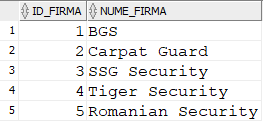
\includegraphics{images/inserare1.png}}
      \caption{ Inserare 1.}
    \end{figure}
    \vspace{0.5cm}
    
    \item \textbf{PROMOVARE}
    \vspace{0.2cm}
    \begin{lstlisting}
CREATE TABLE PROMOVARE (
 id_promovare NUMBER(4) PRIMARY KEY,
 nume_campanie VARCHAR2(50) ,
 data_inceput DATE ,
 data_sfarsit DATE);

INSERT INTO PROMOVARE (id_promovare, nume_campanie, data_inceput, data_sfarsit)
VALUES (1, 'Campania de primavara', TO_DATE('2023-03-15', 'YYYY-MM-DD'), TO_DATE('2023-04-
30', 'YYYY-MM-DD'));
INSERT INTO PROMOVARE (id_promovare, nume_campanie, data_inceput, data_sfarsit)
VALUES (2, 'Campania de reduceri', TO_DATE('2023-09-01', 'YYYY-MM-DD'), TO_DATE('2023-09-15',
'YYYY-MM-DD'));
INSERT INTO PROMOVARE (id_promovare, nume_campanie, data_inceput, data_sfarsit)
VALUES (3, 'Campania de Craciun', TO_DATE('2023-12-10', 'YYYY-MM-DD'), TO_DATE('2023-12-25',
'YYYY-MM-DD'));
INSERT INTO PROMOVARE (id_promovare, nume_campanie, data_inceput, data_sfarsit)
VALUES (4, 'Campania de Paste', TO_DATE('2023-03-01', 'YYYY-MM-DD'), TO_DATE('2023-08-31',
'YYYY-MM-DD'));
INSERT INTO PROMOVARE (id_promovare, nume_campanie, data_inceput, data_sfarsit)
VALUES (5, 'Campania de toamna', TO_DATE('2023-09-15', 'YYYY-MM-DD'), TO_DATE('2023-10-31',
'YYYY-MM-DD'));
    \end{lstlisting} 
    \vspace{0.2cm}
    \begin{figure}[h]
      \centerline{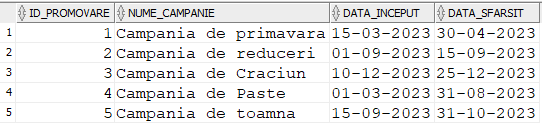
\includegraphics{images/inserare2.png}}
      \caption{ Inserare 2.}
    \end{figure}
    \vspace{0.5cm}

    \item \textbf{MALL}
    \vspace{0.2cm}
    \begin{lstlisting}
CREATE TABLE MALL (
 id_mall NUMBER(4) PRIMARY KEY,
 tara VARCHAR2(50),
 nume_mall VARCHAR2(50),
 dimensiune NUMBER(7),
 id_firma NUMBER(4) NOT NULL,
 id_promovare NUMBER(4),
 FOREIGN KEY (id_firma) REFERENCES FIRMA (id_firma),
 FOREIGN KEY (id_promovare) REFERENCES PROMOVARE (id_promovare)
);
INSERT INTO MALL VALUES (1, 'Romania', 'MegaMall', 10000, 3, 2);
INSERT INTO MALL VALUES (2, 'Spania', 'Plaza Central', 8000, 1, 4);
INSERT INTO MALL VALUES (3, 'Germania', 'City Mall', 12000, 2, 1);
INSERT INTO MALL VALUES (4, 'Franta', 'Le Grand Centre', 15000, 5, 3);
INSERT INTO MALL VALUES (5, 'Italia', 'Fashion Mall', 9000, 4, 5);
INSERT INTO MALL VALUES(6,'Romania','Braila Mall',500,1,null);
    \end{lstlisting}
    \vspace{0.2cm}
    \begin{figure}[h]
      \centerline{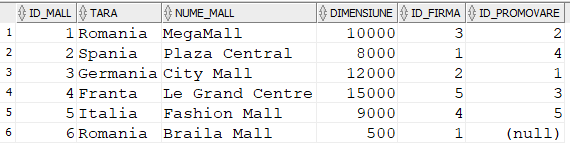
\includegraphics{images/inserare3.png}}
      \caption{ Inserare 3.}
    \end{figure}
    \vspace{0.5cm}

    \item \textbf{CHIRIAS}
    \vspace{0.2cm}
    \begin{lstlisting}
CREATE TABLE CHIRIAS (
 id_chirias NUMBER(4) PRIMARY KEY,
 nume_chirias VARCHAR2(30) ,
 email VARCHAR2(30) NOT NULL
);
INSERT INTO CHIRIAS VALUES (1, 'John Doe', 'john.doe@example.com');
INSERT INTO CHIRIAS VALUES (2, 'Jane Smith', 'jane.smith@example.com');
INSERT INTO CHIRIAS VALUES (3, 'Alex Johnson', 'alex.johnson@example.com');
INSERT INTO CHIRIAS VALUES (4, 'Emily Davis', 'emily.davis@example.com');
INSERT INTO CHIRIAS VALUES (5, 'Michael Brown', 'michael.brown@example.com');
    \end{lstlisting}
    \vspace{0.2cm}
    \begin{figure}[h]
      \centerline{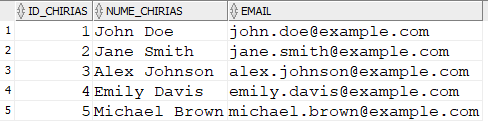
\includegraphics{images/inserare4.png}}
      \caption{ Inserare 4.}
    \end{figure}
    \vspace{0.5cm}

    \item \textbf{MAGAZIN}
    \vspace{0.2cm}
    \begin{lstlisting}
CREATE TABLE MAGAZIN(
 id_magazin NUMBER(4) PRIMARY KEY,
 nume_magazin VARCHAR2(30) ,
 telefon VARCHAR2(30) NOT NULL,
 profit_lunar NUMBER(7),
 id_chirias NUMBER(4) NOT NULL,
 id_mall NUMBER(4) NOT NULL,
 FOREIGN KEY (id_chirias) REFERENCES CHIRIAS (id_chirias),
 FOREIGN KEY (id_mall) REFERENCES MALL (id_mall)
);
INSERT INTO MAGAZIN VALUES (1, 'Carrefour', '123456789', 5000, 1, 1);
INSERT INTO MAGAZIN VALUES (2, 'H and M', '987654321', 7000, 2, 1);
INSERT INTO MAGAZIN VALUES (3, 'New Yorker', '111222333', 6000, 3, 2);
INSERT INTO MAGAZIN VALUES (4, 'Zara', '444555666', 4000, 4, 2);
INSERT INTO MAGAZIN VALUES (5, 'Pull and Bear', '777888999', 8000, 5, 3);
    \end{lstlisting}
    \vspace{0.2cm}
    \begin{figure}[h]
      \centerline{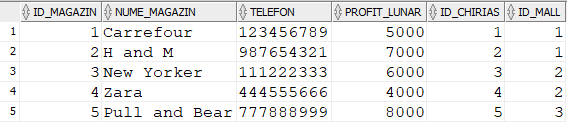
\includegraphics{images/inserare5.png}}
      \caption{ Inserare 5.}
    \end{figure}
    \vspace{0.5cm}

    \item \textbf{STOC}
    \vspace{0.2cm}
    \begin{lstlisting}
CREATE TABLE STOC (
 id_stoc NUMBER(4) PRIMARY KEY,
 id_magazin NUMBER(4),
 FOREIGN KEY (id_magazin) REFERENCES MAGAZIN(id_magazin)
 );

INSERT INTO STOC VALUES (1, 5);
INSERT INTO STOC VALUES (2, 2);
INSERT INTO STOC VALUES (3, 3);
INSERT INTO STOC VALUES (4, 4);
INSERT INTO STOC VALUES (5, 1);
    \end{lstlisting}
    \vspace{4cm}
    \begin{figure}[h]
      \centerline{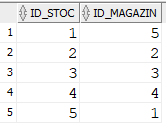
\includegraphics{images/inserare6.png}}
      \caption{ Inserare 6.}
    \end{figure}
    \vspace{0.5cm}

    \item \textbf{TRANZACTIE}
    \vspace{0.2cm}
    \begin{lstlisting}
CREATE TABLE TRANZACTIE(
 id_tranzactie NUMBER(4) PRIMARY KEY,
 data_ora TIMESTAMP,
);
INSERT INTO TRANZACTIE VALUES (1, TIMESTAMP '2023-05-22 14:30:00');
INSERT INTO TRANZACTIE VALUES (2, TIMESTAMP '2023-05-23 09:15:00');
INSERT INTO TRANZACTIE VALUES (3, TIMESTAMP '2023-05-24 16:45:00');
INSERT INTO TRANZACTIE VALUES (4, TIMESTAMP '2023-05-25 12:00:00');
INSERT INTO TRANZACTIE VALUES (5, TIMESTAMP '2023-05-26 18:30:00');
    \end{lstlisting}
    \vspace{0.2cm}
    \begin{figure}[h]
      \centerline{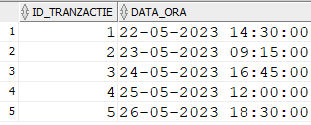
\includegraphics{images/inserare7.png}}
      \caption{ Inserare 7.}
    \end{figure}
    \vspace{0.5cm}

    \item \textbf{PRODUS}
    \vspace{0.2cm}
    \begin{lstlisting}
CREATE TABLE PRODUS (
 id_produs NUMBER(4) PRIMARY KEY,
 nume_produs VARCHAR2(50),
 pret NUMBER(4),
 id_stoc NUMBER(4),
 id_tranzactie NUMBER(4),
 FOREIGN KEY (id_stoc) REFERENCES STOC (id_stoc),
 FOREIGN KEY (id_tranzactie) REFERENCES TRANZACTIE (id_tranzactie)
);
INSERT INTO PRODUS VALUES (1, 'Chec Pufos', 20, 4, 1);
INSERT INTO PRODUS VALUES (2, 'Tricou', 200, 4, 2);
INSERT INTO PRODUS VALUES (3, 'Pantaloni', 300, 3, 2);
INSERT INTO PRODUS VALUES (4, 'Adidasi', 700, 4, 4);
 INSERT INTO PRODUS VALUES (5, 'Lapte', 5, 4, 1);
    \end{lstlisting}
    \vspace{0.2cm}
    \begin{figure}[h]
      \centerline{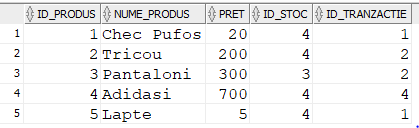
\includegraphics{images/inserare8.png}}
      \caption{ Inserare 8.}
    \end{figure}
    \vspace{0.5cm}

    \item \textbf{CLIENT}
    \vspace{0.2cm}
    \begin{lstlisting}
CREATE TABLE CLIENT (
 id_client NUMBER(4) PRIMARY KEY,
 nume_client VARCHAR2(40),
 email VARCHAR2(30) NOT NULL,
 telefon VARCHAR2(14)
);
INSERT INTO CLIENT VALUES (1, 'Ion Popescu', 'ion.popescu@example.com', '0721122334');
INSERT INTO CLIENT VALUES (2, 'Maria Ionescu', 'maria.ionescu@example.com', '0765432109');
INSERT INTO CLIENT VALUES (3, 'Ana Mihai', 'ana.mihai@example.com', '0755123456');
INSERT INTO CLIENT VALUES (4, 'Mihai Popa', 'mihai.popa@example.com', '0777555888');
INSERT INTO CLIENT VALUES (5, 'Elena Radu', 'elena.radu@example.com', '0744999222');
    \end{lstlisting}
    \vspace{0.2cm}
    \begin{figure}[h]
      \centerline{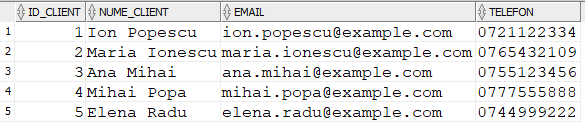
\includegraphics{images/inserare9.png}}
      \caption{ Inserare 9.}
    \end{figure}
    \vspace{0.5cm}

    \item \textbf{RECLAMATIE}
    \vspace{0.2cm}
    \begin{lstlisting}
CREATE TABLE RECLAMATIE (
 id_reclamatie NUMBER(4),
 data_ora TIMESTAMP,
 motiv VARCHAR2(1000),
 id_magazin NUMBER(4),
 id_client NUMBER(4),
 PRIMARY KEY (id_reclamatie, id_magazin, id_client),
 FOREIGN KEY (id_magazin) REFERENCES MAGAZIN (id_magazin),
 FOREIGN KEY (id_client) REFERENCES CLIENT (id_client)
);
INSERT INTO RECLAMATIE VALUES (1, TIMESTAMP '2023-05-22 10:30:00', 'Produs defect', 2, 3);
INSERT INTO RECLAMATIE VALUES (2, TIMESTAMP '2023-05-23 14:45:00', 'Serviciu neadecvat', 1,
4);
INSERT INTO RECLAMATIE VALUES (3, TIMESTAMP '2023-05-24 09:15:00', 'Reclamatie privind
preturile', 3, 2);
INSERT INTO RECLAMATIE VALUES (4, TIMESTAMP '2023-05-25 16:20:00', 'Produsului ii lipseste o
piesa', 1, 1);
INSERT INTO RECLAMATIE VALUES (5, TIMESTAMP '2023-05-26 11:10:00', 'Comportament angajat
neadecvat', 2, 5);
    \end{lstlisting}
    \vspace{0.2cm}
    \begin{figure}[h]
      \centerline{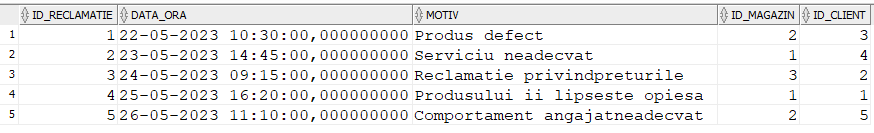
\includegraphics{images/inserare10.png}}
      \caption{ Inserare 10.}
    \end{figure}
    \vspace{0.5cm}

    \item \textbf{ACHIZITIE}
    \vspace{0.2cm}
    \begin{lstlisting}
CREATE TABLE ACHIZITIE (
 id_client NUMBER(4),
 id_magazin NUMBER(4),
 id_tranzactie NUMBER(4),
 PRIMARY KEY (id_client, id_magazin, id_tranzactie),
 FOREIGN KEY (id_magazin) REFERENCES MAGAZIN (id_magazin),
 FOREIGN KEY (id_tranzactie) REFERENCES TRANZACTIE (id_tranzactie),
 FOREIGN KEY (id_client) REFERENCES CLIENT (id_client)
);
INSERT INTO ACHIZITIE VALUES (1, 1, 1);
INSERT INTO ACHIZITIE VALUES (2, 2, 2);
INSERT INTO ACHIZITIE VALUES (3, 1, 3);
INSERT INTO ACHIZITIE VALUES (4, 3, 4);
INSERT INTO ACHIZITIE VALUES (5, 2, 5);
INSERT INTO ACHIZITIE VALUES (4, 1, 2);
INSERT INTO ACHIZITIE VALUES (2, 5, 3);
INSERT INTO ACHIZITIE VALUES (3, 4, 1);
INSERT INTO ACHIZITIE VALUES (5, 2, 4);
INSERT INTO ACHIZITIE VALUES (1, 3, 5);
    \end{lstlisting}
    \vspace{0.2cm}
    \begin{figure}[h]
      \centerline{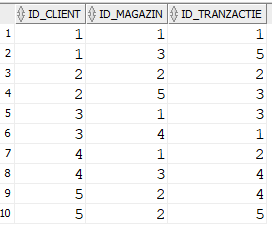
\includegraphics{images/inserare11.png}}
      \caption{ Inserare 11.}
    \end{figure}
    \vspace{0.5cm}

    \item \textbf{ANGAJAT}
    \vspace{0.2cm}
    \begin{lstlisting}
CREATE TABLE ANGAJAT (
 id_angajat NUMBER(4) PRIMARY KEY,
 nume_angajat VARCHAR2(30),
 salariu NUMBER(4),
 data_angajarii DATE
);
INSERT INTO ANGAJAT VALUES(1, 'Ion Popescu', 3000, TO_DATE('2022-01-15', 'YYYY-MM-DD'));
INSERT INTO ANGAJAT VALUES(2, 'Maria Ionescu', 2500, TO_DATE('2022-02-01', 'YYYY-MM-DD'));
INSERT INTO ANGAJAT VALUES(3, 'Alexandru Stanescu', 3500, TO_DATE('2022-03-10', 'YYYY-MMDD'));
INSERT INTO ANGAJAT VALUES(4, 'Elena Dumitrescu', 2800, TO_DATE('2022-04-05', 'YYYY-MM-DD'));
INSERT INTO ANGAJAT VALUES(5, 'Mihai Radu', 3200, TO_DATE('2022-05-20', 'YYYY-MM-DD'));
INSERT INTO ANGAJAT VALUES(6, 'Ana Vasilescu', 2700, TO_DATE('2022-06-11', 'YYYY-MM-DD'));
INSERT INTO ANGAJAT VALUES(7, 'Constantin Moldovan', 2900, TO_DATE('2022-07-02', 'YYYY-MMDD'));
INSERT INTO ANGAJAT VALUES(8, 'Andreea Nicolescu', 3100, TO_DATE('2022-08-18', 'YYYY-MM-DD'));
INSERT INTO ANGAJAT VALUES(9, 'George Marin', 2600, TO_DATE('2022-09-07', 'YYYY-MM-DD'));
INSERT INTO ANGAJAT VALUES(10, 'Simona Gheorghe', 3000, TO_DATE('2022-10-25', 'YYYY-MM-DD'));
INSERT INTO ANGAJAT VALUES(11,'Razvan Marian', 3500, TO_DATE('2018-05-29', 'YYYY-MM-DD'));
    \end{lstlisting}
    \vspace{0.2cm}
    \begin{figure}[h]
      \centerline{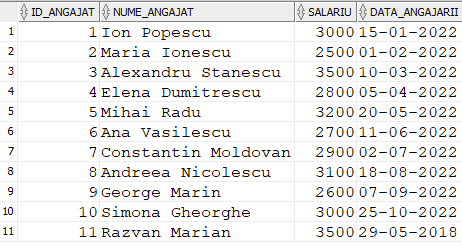
\includegraphics{images/inserare12.png}}
      \caption{ Inserare 12.}
    \end{figure}
    \vspace{0.5cm}

    \item \textbf{PAZNIC}
    \vspace{0.2cm}
    \begin{lstlisting}
CREATE TABLE PAZNIC (
 id_paznic NUMBER(4),
 norma VARCHAR2(20),
 id_angajat NUMBER(4) UNIQUE,
 id_firma NUMBER(4),
 PRIMARY KEY (id_angajat, id_paznic),
 FOREIGN KEY (id_angajat) REFERENCES ANGAJAT (id_angajat),
 FOREIGN KEY (id_firma) REFERENCES FIRMA (id_firma)
);
INSERT INTO PAZNIC VALUES(1, 'Norma intreaga', 1,1);
INSERT INTO PAZNIC VALUES(2, 'Norma intreaga', 3,2);
INSERT INTO PAZNIC VALUES(3, 'Part-time', 2,2);
INSERT INTO PAZNIC VALUES(4, 'Part-time', 5,3);
INSERT INTO PAZNIC VALUES(5, 'Norma intreaga', 4,5);
INSERT INTO PAZNIC VALUES(6,'Norma intreaga', 11, 3);
    \end{lstlisting}
    \vspace{0.2cm}
    \begin{figure}[h]
      \centerline{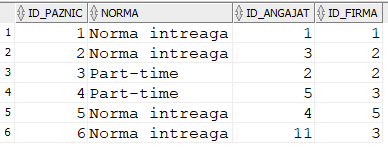
\includegraphics{images/inserare13.png}}
      \caption{ Inserare 13.}
    \end{figure}
    \vspace{0.5cm}

    \item \textbf{INTERN}
    \vspace{0.2cm}
    \begin{lstlisting}
CREATE TABLE INTERN (
 id_intern NUMBER(4),
 tura VARCHAR2(20),
 id_angajat NUMBER(4) UNIQUE,
 PRIMARY KEY (id_angajat, id_intern),
 id_magazin NUMBER(4),
 FOREIGN KEY (id_angajat) REFERENCES ANGAJAT (id_angajat),
 FOREIGN KEY (id_magazin) REFERENCES MAGAZIN (id_magazin)
);
INSERT INTO INTERN VALUES(1, 'Zi', 6,1);
INSERT INTO INTERN VALUES(2, 'Zi', 8,2);
INSERT INTO INTERN VALUES(3, 'Noapte', 7,3);
INSERT INTO INTERN VALUES(4, 'Noapte', 10,4);
INSERT INTO INTERN VALUES(5, 'Noapte', 9,5);
    \end{lstlisting}
    \vspace{0.2cm}
    \begin{figure}[h]
      \centerline{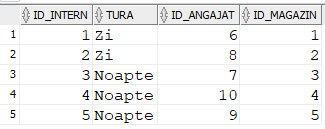
\includegraphics{images/inserare14.png}}
      \caption{ Inserare 14.}
    \end{figure}
    \vspace{0.5cm}
\end{itemize}
